%!TEX root = ../RelazioneStrutturaleMeoliNicola.tex
\chapter{Relazione strutturale}
La presente relazione contiene lo svolgimento del calcolo delle sollecitazione a momento e taglio e il calcolo dello sforzo assiale massimo rispettivamente di una trave e di due pilastri di un edificio composto da 4 piani di cui 3 fuori terra situato in provincia di Trento ad un'altitudine di \SI{300}{\meter} sopra il livello del mare.

Di seguito si riassumono brevemente le caratteristiche presenti nel progetto strutturale dell'edificio, distribuito all'interno della domanda del committente.
Verranno analizzati meglio gli strati nei capitoli successivi, man mano che serviranno nei calcoli.
\section{Composizione dell'edificio}
La struttura è a telaio in calcestruzzo armato, caratterizzata da pilastri quadrati di sezione \SI{30}{\centi\meter} e da travi sia a spessore che non, rispettivamente larghe \SI{60}{\centi\meter} ed alte come lo spessore del solaio, e $30 \times \SI{50}{\centi\metre}$.

I solai strutturali sono di tipo a lastre tralicciate Predalle tra il piano interrato e il piano terra e nel solaio di copertura. 
Il peso ultimato di tale solaio di \SI{3.6}{\kilo\newton\per\square\meter}.
I solai tra piano terra e piano primo e tra piano primo e piano secondo sono di tipo a travetti e latero-cemento.
Il peso ultimato di tale solaio di \SI{3.20}{\kilo\newton\per\square\meter}.

I solai dei piano intermedi sono costituiti da un pacchetto con calcestruzzo alleggerito, massetto di allettamento, intonaco e pavimento in ceramica.
Il solaio nella zona del terrazzo è costituito da isolante, impermealizzazione, massetto in calcestruzzo e pavimento.
Il solaio di copertura è costituito da isolante, massetto in calcestruzzo alleggerito, impermealizzazione e ghiaia.

Le pareti divisorie interne sono costituite da muratura in laterizio e intonaco in ambo i lati.
Le pareti perimetrali sono costituite da muratura in laterizio, cappotto esterno e intonaco.

Il piano terra è adibito a negozi, il piano primo ad uffici aperti al pubblico, il piano secondo a civile abitazione.
Il piano interrato è adibito a garage.

\section{Normativa di riferimento e coefficienti utilizzati}
Sono state utilizzate le normative attualmente in vigore in Italia, in particolare 
\begin{itemize}
\item \norma{Decreto Ministeriale 17 gennaio 2018}, d'ora in poi chiamato \norma{NTC2018}
\item \norma{Circolare 21 gennaio 2019 n. 7, C.S.LL.PP}, d'ora in poi chiamata \norma{circolare}
\end{itemize}
Nel calcolo delle combinazioni di carico agli SLU e SLE sono stati utilizzati i coefficienti di combinazione e i coefficienti parziali in \normaref{Tab\,2.5.I} ed in \normaref{Tab\,2.6.I} riportati dalle \norma{NTC2018}.
Vengono riportati per comodità in questo capitolo.
\clearpage
\begin{figure*}[htb]
\subfloat{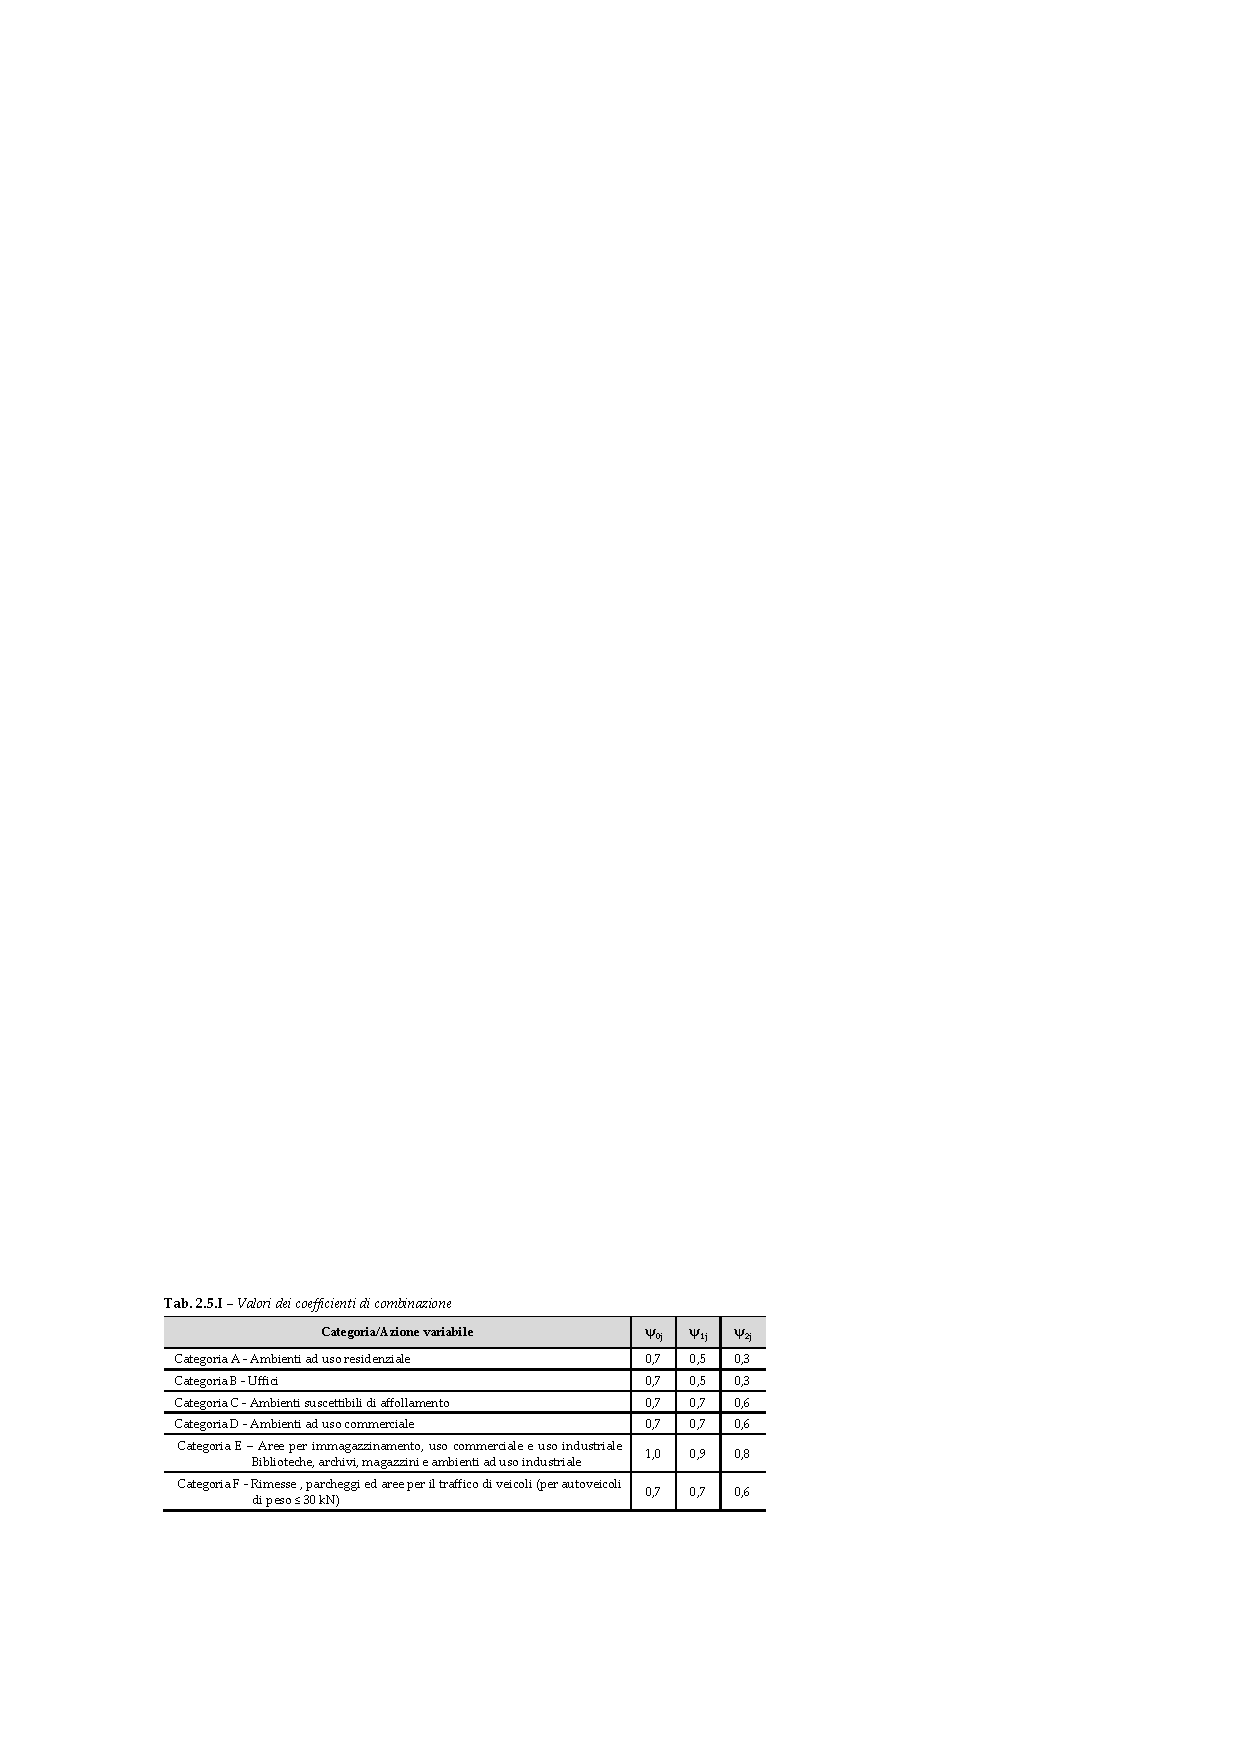
\includegraphics[width=0.55\textwidth,valign=t]{IMG/tab2-5-I.pdf}} 
\subfloat{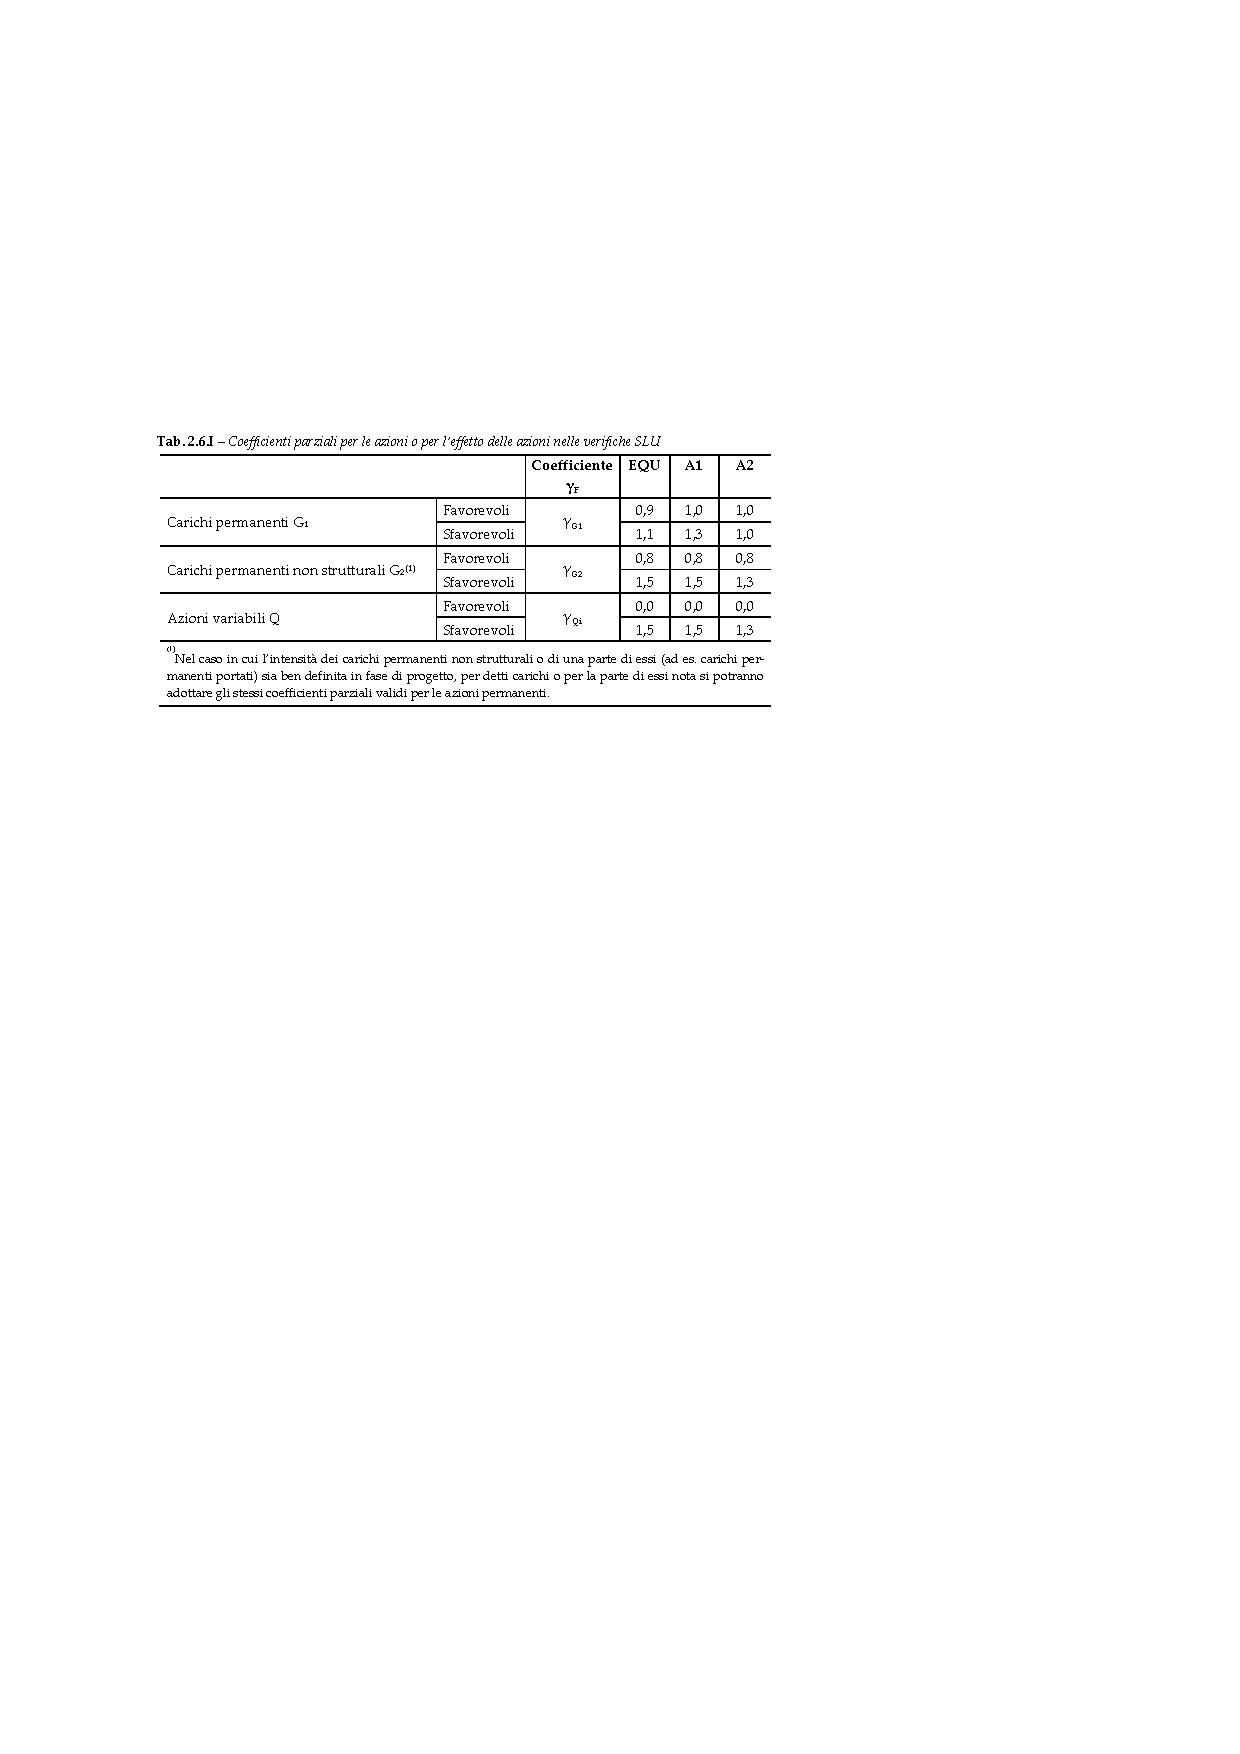
\includegraphics[width=0.45\textwidth,valign=t]{IMG/tab2-6-I.pdf}}\\
\subfloat{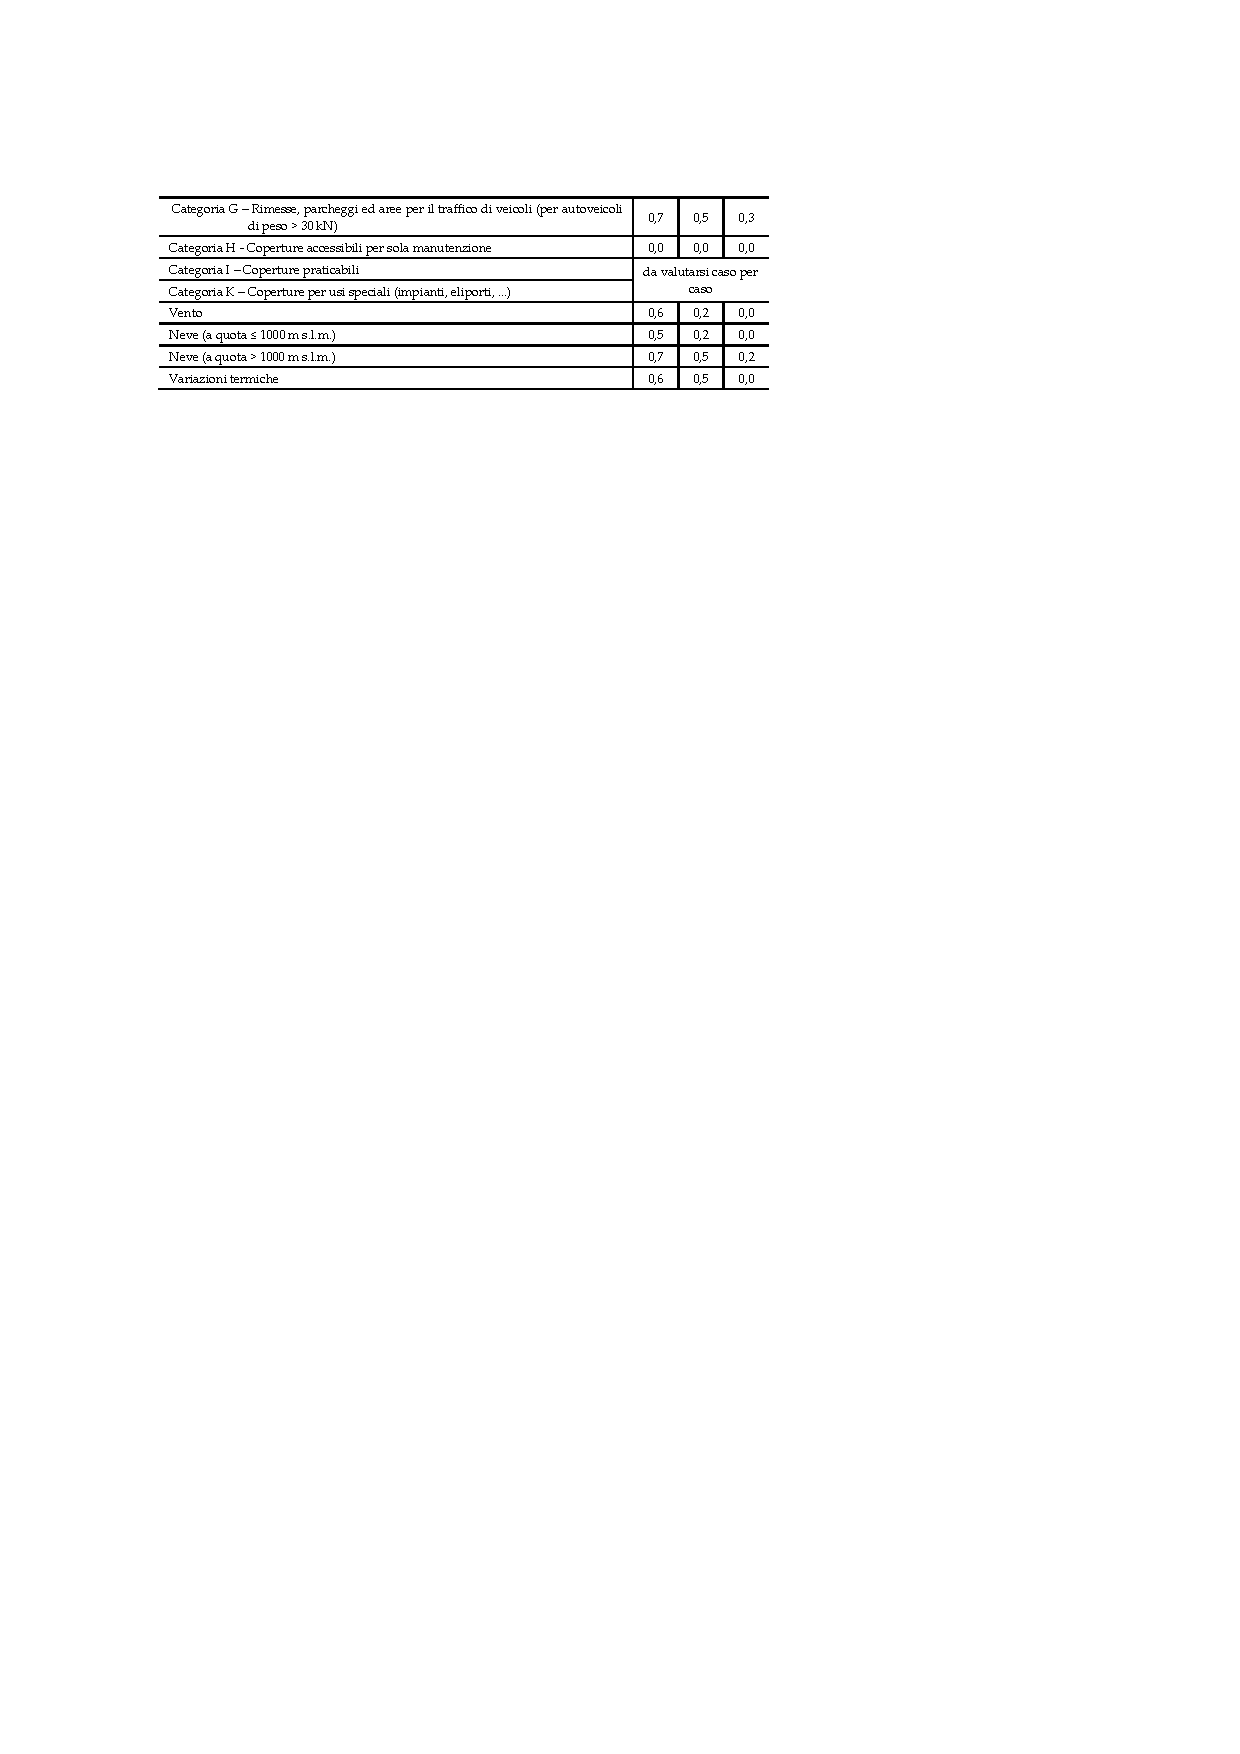
\includegraphics[width=0.55\textwidth]{IMG/tab2-5-I-2.pdf}} 
\end{figure*}
\section{Criteri stilistici adottati nella presente relazione}
Per maggior chiarezza di lettura si vogliono qui esplicare i diversi tipi di carattere che sono presenti all'interno di queste pagine.
\paragraph*{Numeri di figure e tabelle nelle didascalie} Per distinguere meglio i nomi che figure e tabelle hanno: con il \textbf{Testo in nero} sono riportati direttamente le immagini prese dalle rispettive norme; con il \textcolor{myGray}{Testo in grigio} sono riportati figure e tabelle create appositamente per questa relazione.
\paragraph*{Richiami ad elementi presenti nelle normative} Con \normaref{questo carattere} utilizzato all'interno dei testi che seguiranno si intende richiamare figure, tabelle o paragrafi presenti nelle normative (richiamate con \norma{questo carattere}).
Con il carattere normale vengono invece richiamati gli elementi creati appositamente in questa relazione (figure, tabelle o formule).
